\documentclass[12pt,letterpaper, onecolumn]{exam}
\usepackage{amsmath}
\usepackage{amssymb}
\usepackage[lmargin=71pt, tmargin=1.2in]{geometry}  %For centering solution box
\usepackage[shortlabels]{enumitem}
\usepackage{subcaption}
\usepackage[final]{graphicx}
\lhead{Leaft Header\\}
\rhead{Right Header\\}
% \chead{\hline} % Un-comment to draw line below header
\thispagestyle{empty}   %For removing header/footer from page 1

\begin{document}

\begingroup  
    \centering
    \LARGE Machine Learning: Project\\
    \LARGE Multi-Agent Learning in Canonical Games and Knights Archers Zombies\\[0.5em]
    \large \today\\[0.5em]
    \large Dimitrios Mystriotis - Jan Cichomski\par
    \large r1027781 - r1026448\par
\endgroup
\rule{\textwidth}{0.4pt}
\pointsdroppedatright   %Self-explanatory
\printanswers
\renewcommand{\solutiontitle}{\noindent\textbf{Ans:}\enspace}   %Replace "Ans:" with starting keyword in solution box

\section{\textbf{Task 1:}}

\section{\textbf{Task 2:}}
\subsection{}
\begin{itemize}
    \item A game is in Nash equilibrium when no player can improve their outcome by changing their strategy, if the other player doesn't change their's.
    \item A game is in Pareto Optimal when it is impossible to make a player better off without making the total payoff worse.
\end{itemize}
\begin{enumerate}[(\alph*)]
    \item Stag Hunt:
    \begin{itemize}
        \item Nash Equilibria: (Hare,Hare) and (Stag,Stag)
        \item Pareto Optimal: (Hare,Hare) and (Stag,Stag)
    \end{itemize}
    \item Subsidy game:
    \begin{itemize}
        \item Nash Equilibria: (Subsidy 2,Subsidy 2)
        \item Pareto Optimal: (Subsidy 1,Subsidy 1) and (Subsidy 2,Subsidy 2)
    \end{itemize}
    \item Matching Pennis:
    \begin{itemize}
        \item Nash Equilibria: There is no Nash Equilibria for a pure strategy. For a mixed strategy, the Nash Equilibria is picking heads or tails with probability 0.5 each.
        \item Pareto Optimal: Every outcome is Pareto Optimal
    \end{itemize}
    \item Prisoner's Dilemma:
    \begin{itemize}
        \item Nash Equilibria: (Defect,Defect)
        \item Pareto Optimal: (Cooperate,Cooperate)
    \end{itemize}
\end{enumerate}

\subsection{}

The e-Greedy algorithm converges to the Nash Equilibrium for all games. Even when an algorithm converges to the Pareto Optimal solution, it starts to move towards the Nash Equilibrium
as the number of iterations increases. This is because the Nash Equilibrium is the most stable solution, which random choices will favor. The values plotted are the q-values of the agents
and so each of the quarters represents a game outcome as the agents pick the action with the highest q-value deterministically.

\begin{figure}
    \begin{subfigure}{.5\textwidth}
      \centering
      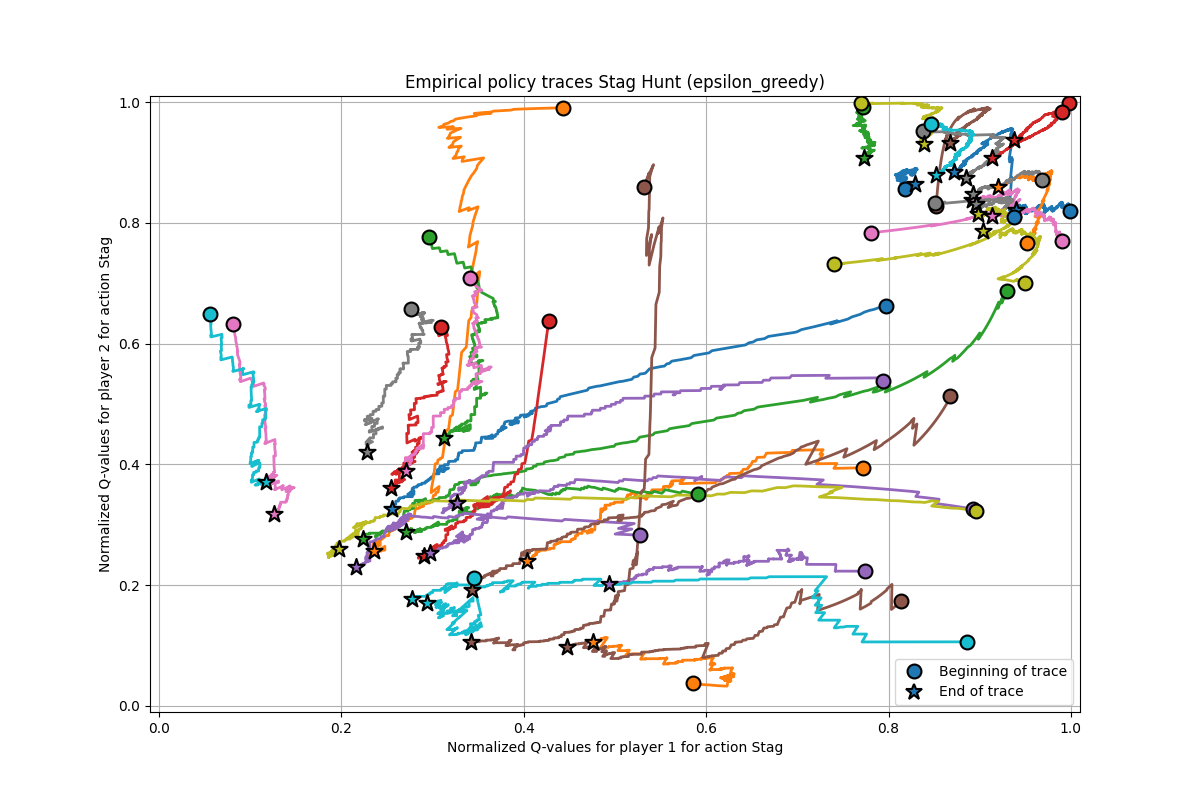
\includegraphics[width=.6\linewidth]{plots/replicator_trajectoreis_Stag Hunt_epsilon_greedy.png}
      \caption{e-Greedy Stag Hunt}
      \label{fig:sfigesh}
    \end{subfigure}%
    \begin{subfigure}{.5\textwidth}
      \centering
      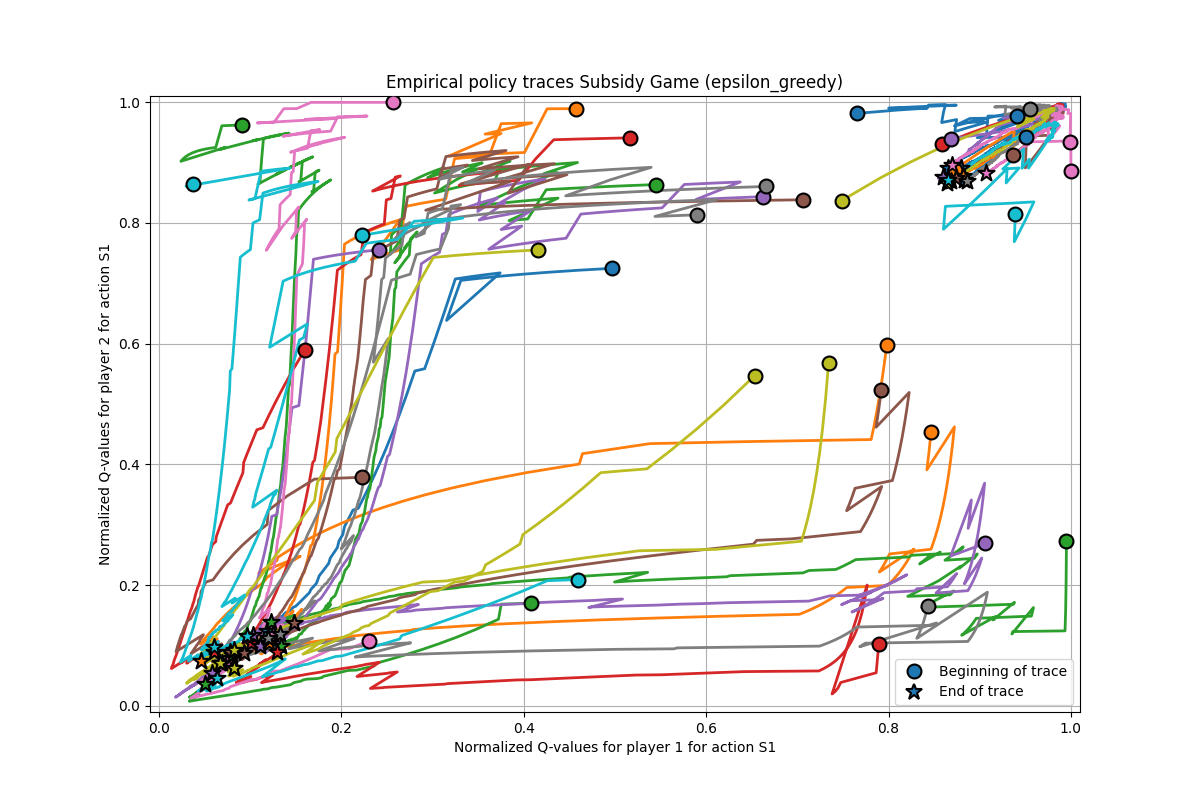
\includegraphics[width=.6\linewidth]{plots/replicator_trajectoreis_Subsidy Game_epsilon_greedy.png}
      \caption{e-Greedy Subsidy Game}
      \label{fig:sfigesg}
    \end{subfigure}\\
    \begin{subfigure}{.5\textwidth}
      \centering
      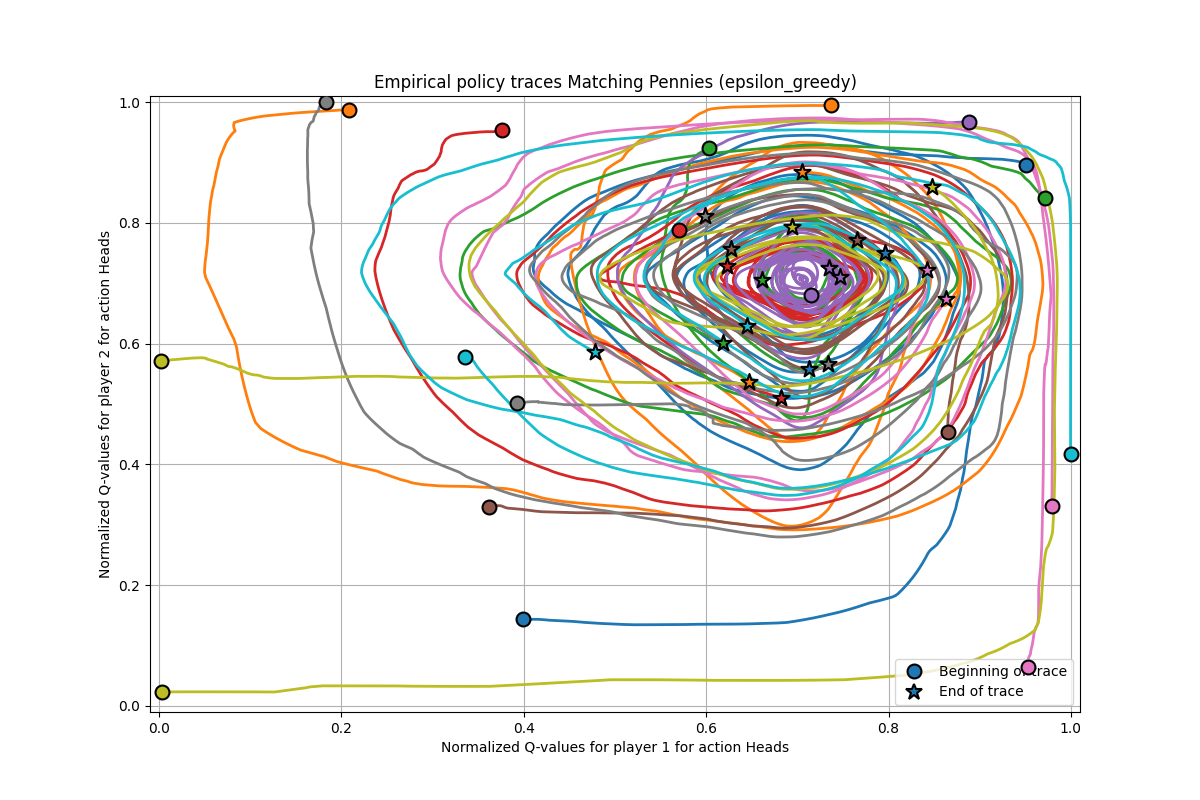
\includegraphics[width=.6\linewidth]{plots/replicator_trajectoreis_Matching Pennies_epsilon_greedy.png}
      \caption{e-Greedy Matching Pennies}
      \label{fig:sfigemp}
    \end{subfigure}%
    \begin{subfigure}{.5\textwidth}
      \centering
      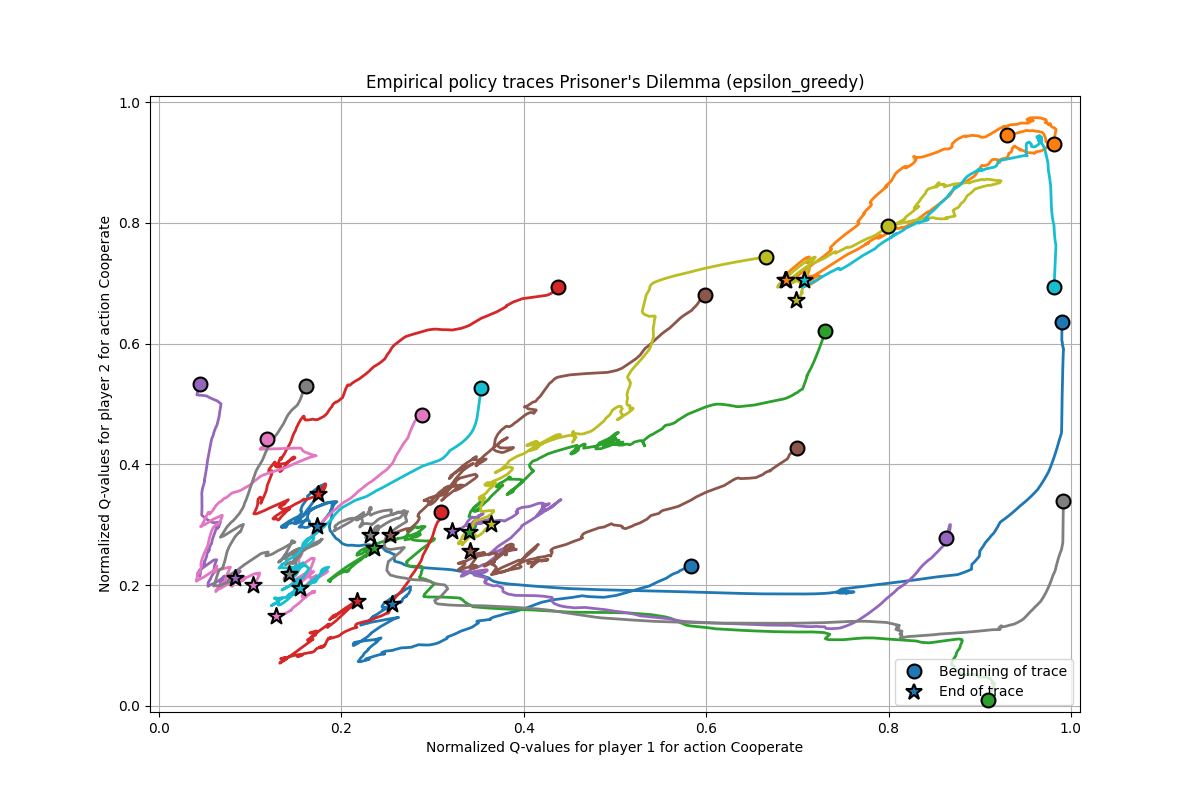
\includegraphics[width=.6\linewidth]{plots/replicator_trajectoreis_Prisoner's Dilemma_epsilon_greedy.png}
      \caption{e-Greedy Prisoner's Dilemma}
      \label{fig:sfigepd}
    \end{subfigure}%
\end{figure}

The Boltzmann algorithm converges to either the Nash Equilibrium or the Pareto Optimal solution. The Boltzmann algorithm is more likely to converge to the Pareto Optimal solution
compared to the e-Greedy algorithm, and it doesn't deviate from that point. The algorithm will basically find an optimal solution (either Nash or Pareto) and stick to it.
Which on is favored depends on the starting distance from the point and the rewards of the game. It seams to favor the Nash Equilibrium slightly more than the Pareto Optimal solution.

\begin{figure}
    \begin{subfigure}{.5\textwidth}
      \centering
      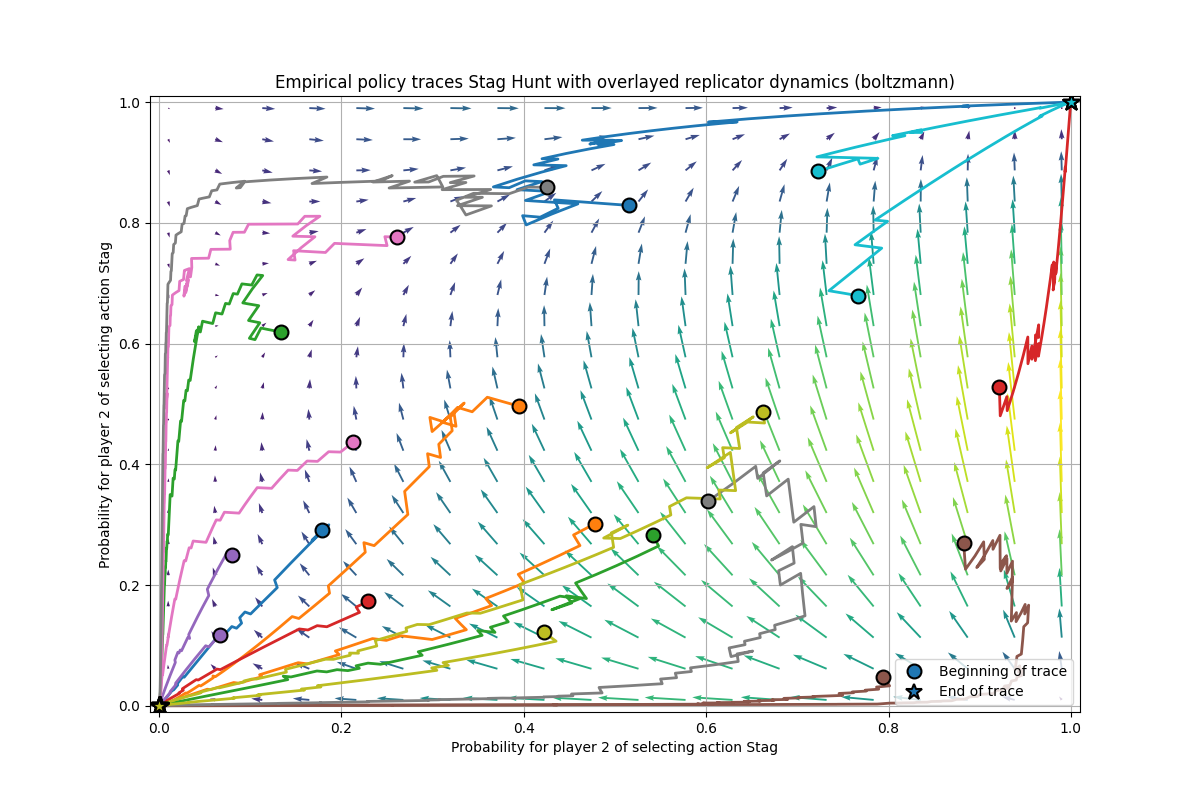
\includegraphics[width=.6\linewidth]{plots/replicator_trajectoreis_Stag Hunt_boltzmann.png}
      \caption{Boltzmann Q-Learning Stag Hunt}
      \label{fig:sfigbsh}
    \end{subfigure}%
    \begin{subfigure}{.5\textwidth}
      \centering
      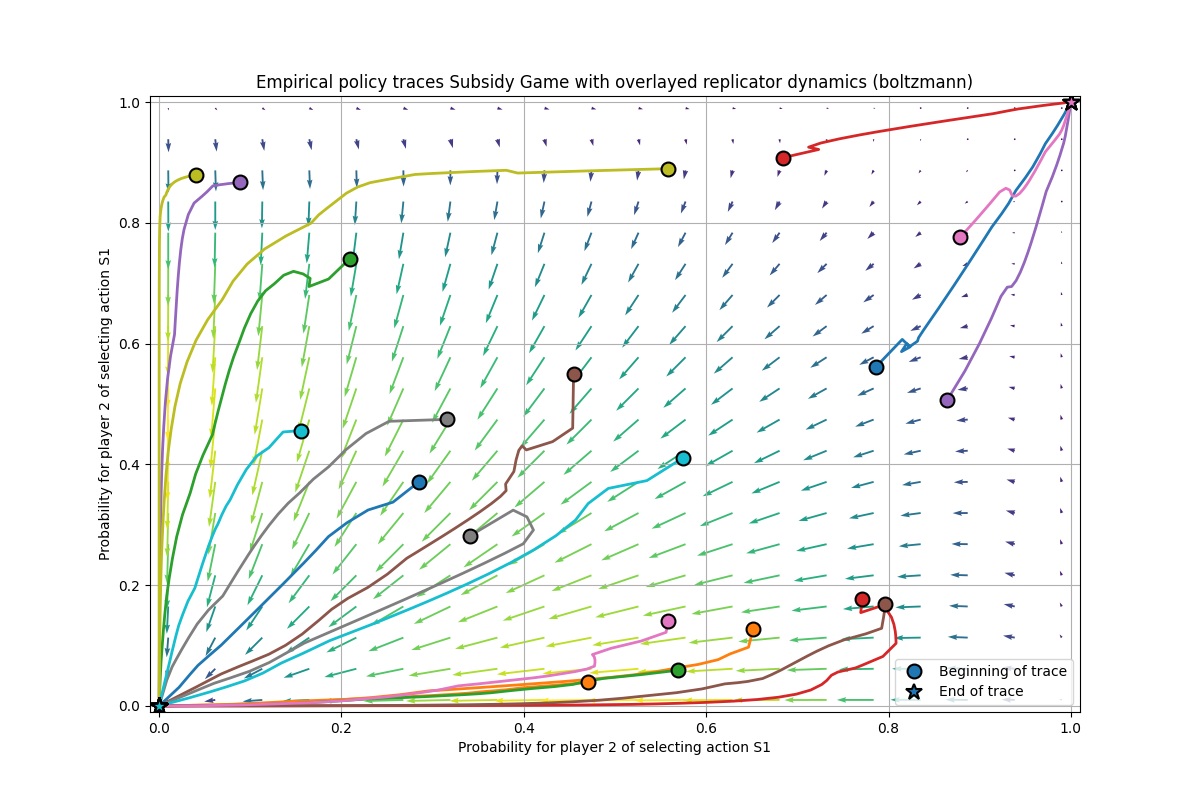
\includegraphics[width=.6\linewidth]{plots/replicator_trajectoreis_Subsidy Game_boltzmann.png}
      \caption{Boltzmann Q-Learning Subsidy Game}
      \label{fig:sfigbsg}
    \end{subfigure}\\
    \begin{subfigure}{.5\textwidth}
      \centering
      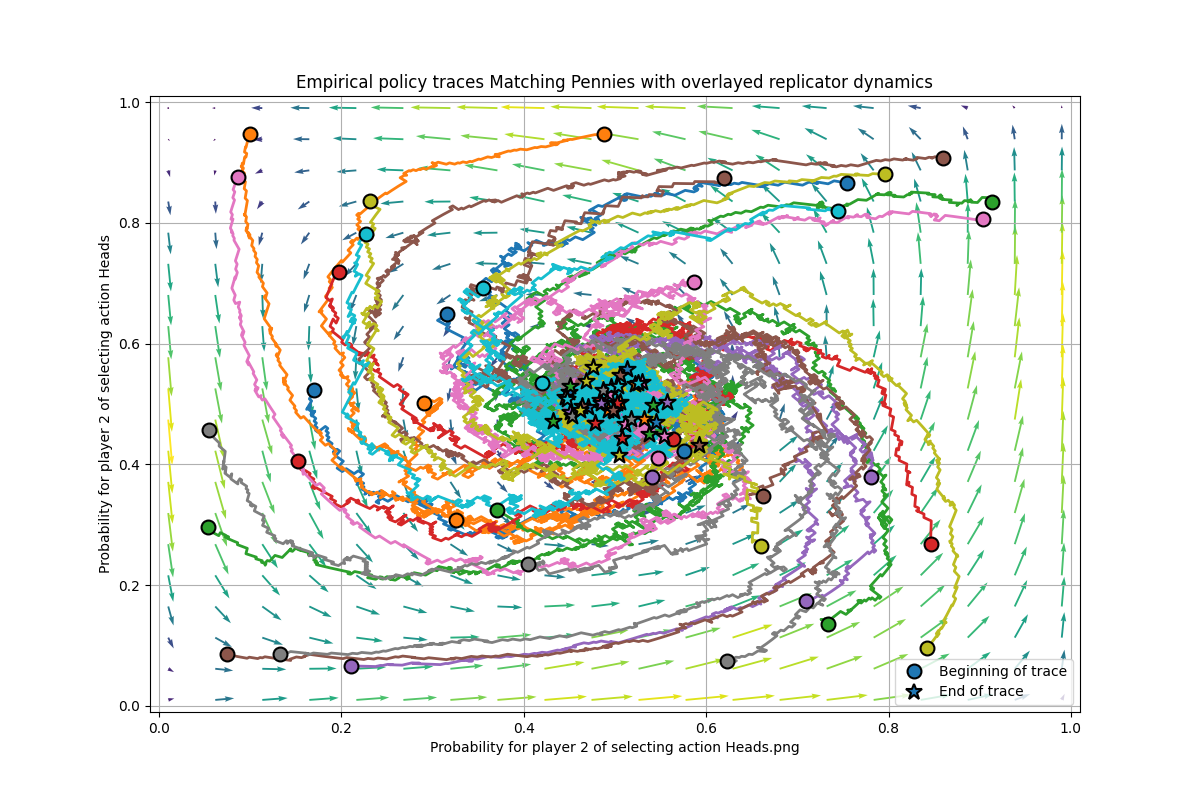
\includegraphics[width=.6\linewidth]{plots/replicator_trajectoreis_Matching Pennies_boltzmann.png}
      \caption{Boltzmann Q-Learning Matching Pennies}
      \label{fig:sfigbmp}
    \end{subfigure}%
    \begin{subfigure}{.5\textwidth}
      \centering
      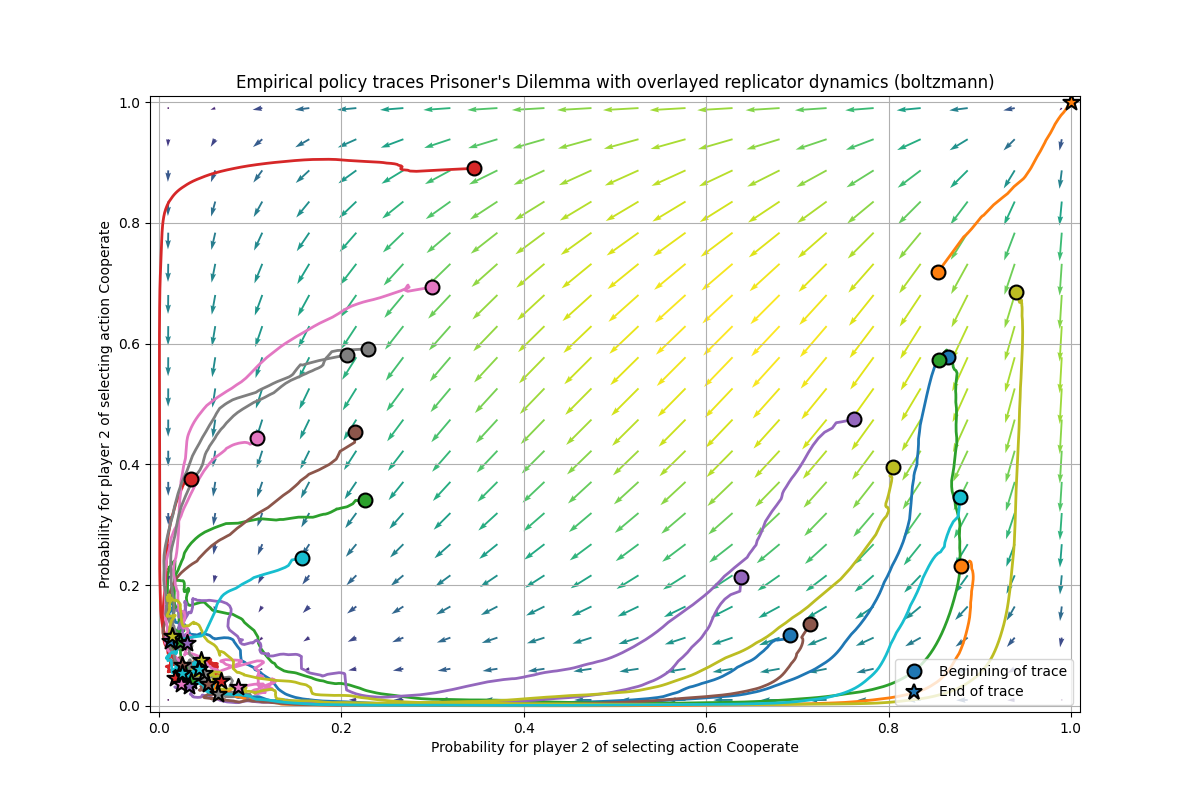
\includegraphics[width=.6\linewidth]{plots/replicator_trajectoreis_Prisoner's Dilemma_boltzmann.png}
      \caption{Boltzmann Q-Learning Prisoner's Dilemma}
      \label{fig:sfigbpd}
    \end{subfigure}%
\end{figure}

For the Lenient Boltzmann Q-Learning algorithm, the results are similar to the Boltzmann Q-Learning algorithm. The main advantage of the Lenient Boltzmann Q-Learning algorithm is that it
allow for more exploration, by allowing for some suboptimal choices. This can be seen in the plots, where the algorithm is more likely to explore the state space and find the Pareto Optimal solution.
The existence of the k value allow for the algorithm to explore more or less, depending on the value of k.

\begin{figure}
    \begin{subfigure}{.5\textwidth}
      \centering
      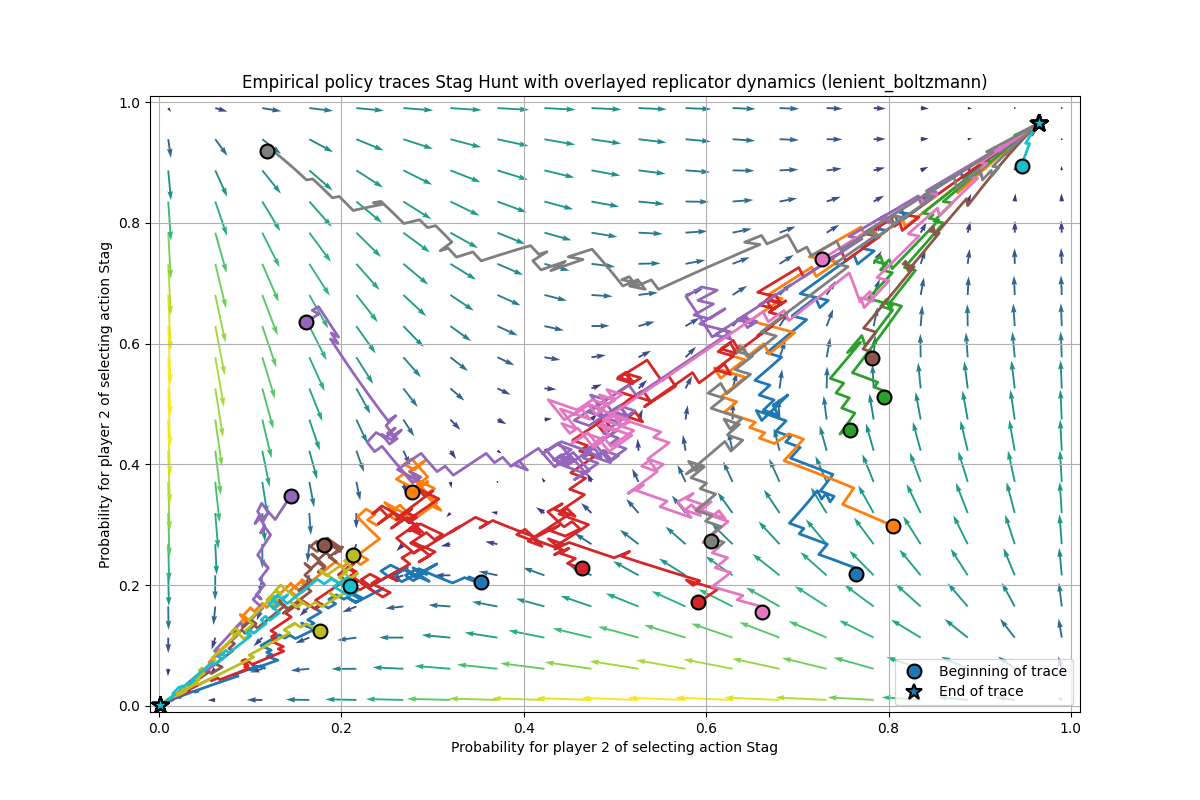
\includegraphics[width=.6\linewidth]{plots/replicator_trajectoreis_Stag Hunt_lenient_boltzmann.png}
      \caption{Lenient Boltzmann Q-Learning\\ Stag Hunt}
      \label{fig:sfiglbsh}
    \end{subfigure}%
    \begin{subfigure}{.5\textwidth}
      \centering
      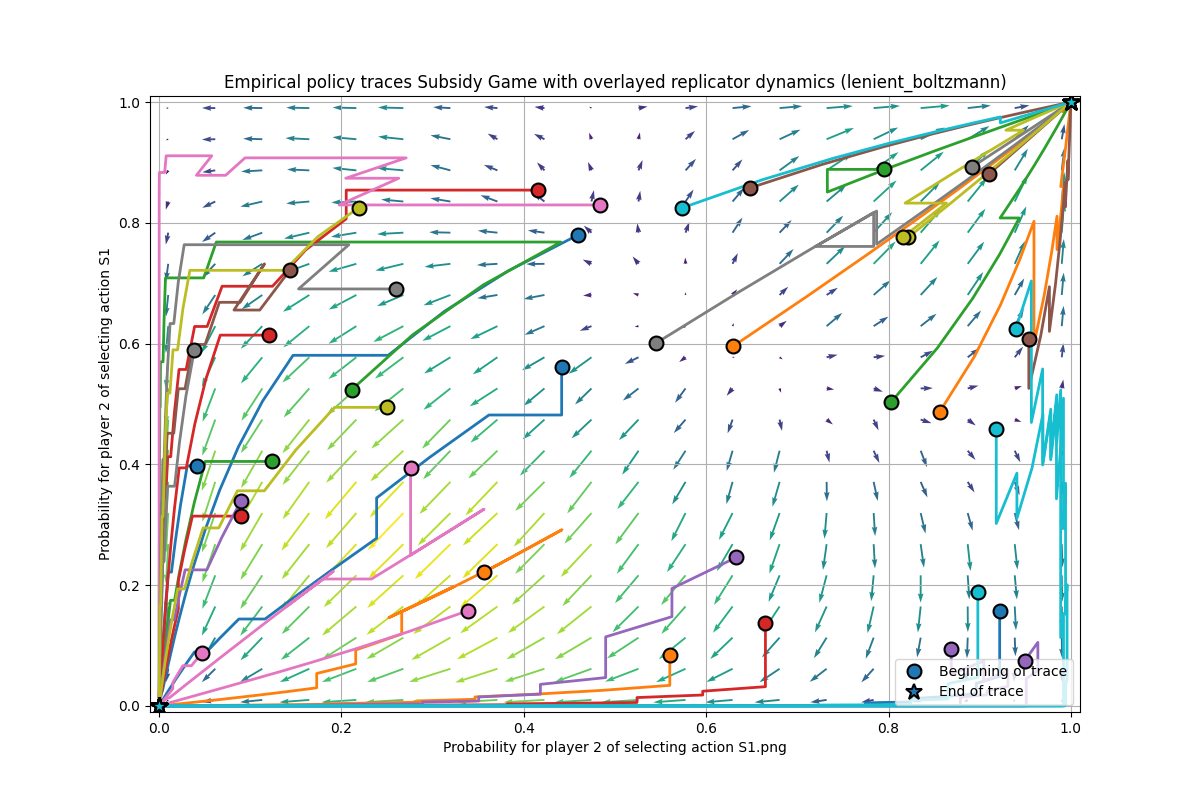
\includegraphics[width=.6\linewidth]{plots/replicator_trajectoreis_Subsidy Game_lenient_boltzmann.png}
      \caption{Lenient Boltzmann Q-Learning\\ Subsidy Game}
      \label{fig:sfiglbsg}
    \end{subfigure}\\
    \begin{subfigure}{.5\textwidth}
      \centering
      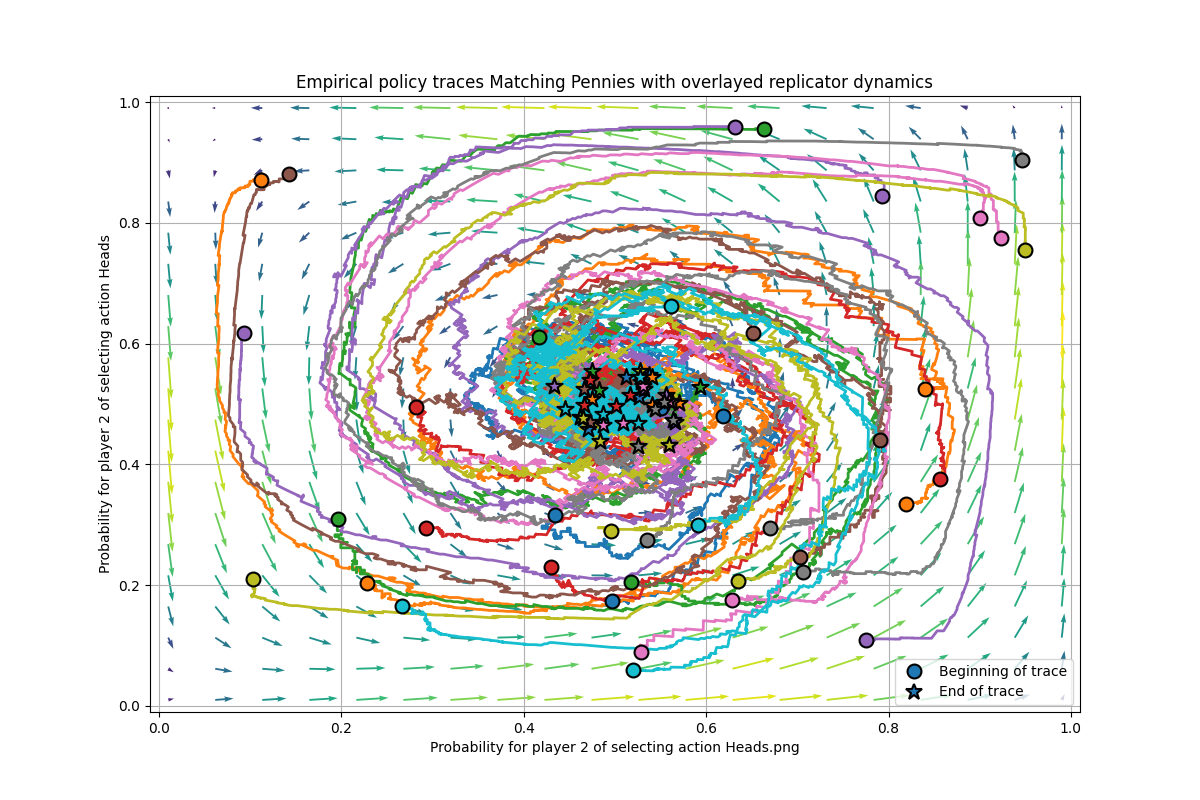
\includegraphics[width=.6\linewidth]{plots/replicator_trajectoreis_Matching Pennies_lenient_boltzmann.png}
      \caption{Lenient Boltzmann Q-Learning\\ Matching Pennies}
      \label{fig:sfiglbmp}
    \end{subfigure}%
    \begin{subfigure}{.5\textwidth}
      \centering
      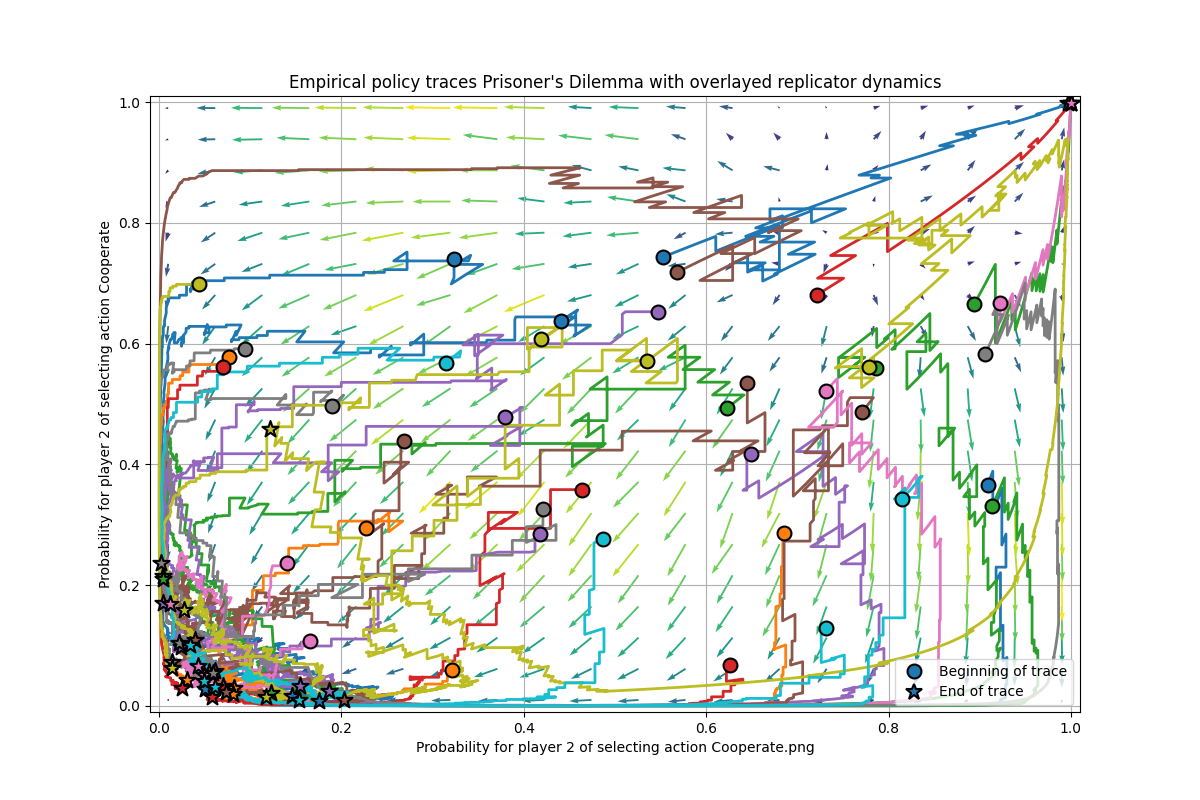
\includegraphics[width=.6\linewidth]{plots/replicator_trajectoreis_Prisoner's Dilemma_lenient_boltzmann.png}
      \caption{Lenient Boltzmann Q-Learning\\ Prisoner's Dilemma}
      \label{fig:sfiglbpd}
    \end{subfigure}%
\end{figure}
\subsection{}

\section{\textbf{Task 3:}}

\section{\textbf{Task 4:}}


\end{document}